\documentclass[aspectratio=169,10pt]{beamer}

\usepackage[T1]{fontenc}
\usepackage[utf8]{inputenc}
\usepackage[indonesian]{babel}
\usepackage{amsmath}
\usepackage{amssymb}
\usepackage{tikz}
\usepackage{ragged2e}
\usepackage{array}
\usepackage{graphicx}
\usepackage{hyperref}
\usepackage{booktabs}

\usetikzlibrary{arrows.meta,calc,fit,positioning,shapes.geometric,backgrounds}

\graphicspath{{assets/}}

\definecolor{Ink}{HTML}{13293D}
\definecolor{Sky}{HTML}{3E7B9C}
\definecolor{Mist}{HTML}{EAF1F6}
\definecolor{Leaf}{HTML}{DDF0D8}
\definecolor{Sand}{HTML}{FFF2CC}
\definecolor{Rose}{HTML}{F8D7DA}
\definecolor{Slate}{HTML}{5C6770}
\definecolor{SoftBlue}{HTML}{D9E8F5}

\setbeamertemplate{navigation symbols}{}
\setbeamertemplate{footline}[frame number]
\setbeamertemplate{blocks}[rounded][shadow=false]
\setbeamertemplate{itemize item}{\color{Sky}$\blacktriangleright$}
\setbeamertemplate{itemize subitem}{\color{Sky}$\bullet$}
\setbeamertemplate{enumerate item}{\color{Sky}\bfseries\insertenumlabel.}

\setbeamercolor{background canvas}{bg=white}
\setbeamercolor{normal text}{fg=Ink,bg=white}
\setbeamercolor{frametitle}{fg=Ink,bg=white}
\setbeamercolor{framesubtitle}{fg=Slate}
\setbeamercolor{title}{fg=Ink}
\setbeamercolor{block title}{fg=white,bg=Ink}
\setbeamercolor{block body}{fg=Ink,bg=Mist}
\setbeamercolor{footline}{fg=Ink,bg=white}

\setbeamerfont{title}{size=\Large,series=\bfseries}
\setbeamerfont{frametitle}{size=\Large,series=\bfseries}
\setbeamerfont{framesubtitle}{size=\small,shape=\itshape}
\setbeamerfont{block title}{series=\bfseries}

\newcommand{\pill}[2]{%
  \tikz[baseline=(n.base)]\node[rounded corners=8pt, fill=#1, text=Ink, inner xsep=7pt, inner ysep=3pt] (n) {\scriptsize #2};%
}

\newcommand{\sectiontitle}[1]{%
  {\large\bfseries #1}%
}

\begin{document}

% ─────────────────────────────────────────────
%  SLIDE 1 · Judul
% ─────────────────────────────────────────────
\begin{frame}[plain]
  \begin{tikzpicture}[remember picture,overlay]
    \fill[Ink!8]  ([xshift=4.3cm, yshift=-4.8cm]current page.north west) circle (1.2cm);
    \fill[Ink!6]  ([xshift=9.8cm, yshift=-6.4cm]current page.north west) circle (2.1cm);
    \fill[Sky!20] ([xshift=14.5cm,yshift=-2.0cm]current page.north west) circle (1.8cm);
    \fill[Sky!10] ([xshift=1.0cm, yshift=-7.5cm]current page.north west) circle (1.0cm);
  \end{tikzpicture}

  \vfill
  \begin{center}
    \begin{minipage}{0.82\textwidth}
      \centering

      {\color{Sky}\rule{4cm}{2pt}}

      \vspace{0.30cm}
      {\usebeamerfont{title}
        Penerapan \textit{Particle Swarm Optimization} (PSO)\\[5pt]
        untuk \textit{Traveling Salesperson Problem} (TSP)
      \par}

      \vspace{0.15cm}
      {\color{Slate}\small Studi Kasus: Kabupaten/Kota di Jawa Barat}

      \vspace{0.40cm}
      {\color{Sky}\rule{4cm}{1pt}}

      \vspace{0.30cm}
      \begin{tabular}{@{}ll@{\hspace{1.4cm}}ll@{}}
        {\color{Ink}\footnotesize Naufal Akmal Rizqulloh} & {\color{Slate}\footnotesize G6401231065} &
        {\color{Ink}\footnotesize Insan Anshary Rasul}    & {\color{Slate}\footnotesize G6401231132} \\[4pt]
        {\color{Ink}\footnotesize Adhiya Radhin Fasya}    & {\color{Slate}\footnotesize G6401231068} &
        {\color{Ink}\footnotesize Daffa Naufal Mumtaz}    & {\color{Slate}\footnotesize G6401231168} \\[4pt]
        {\color{Ink}\footnotesize Faiz Naufal Huda}       & {\color{Slate}\footnotesize G6401231124} & & \\
      \end{tabular}

      \vspace{0.35cm}
      {\color{Slate}\small
        Departemen Ilmu Komputer
        $\cdot$ Institut Pertanian Bogor
        $\cdot$ 2026
      }
    \end{minipage}
  \end{center}
  \vfill
\end{frame}


% ─────────────────────────────────────────────
%  SLIDE 2 · Gambaran Project
% ─────────────────────────────────────────────
\begin{frame}{Gambaran Project}
  \framesubtitle{Naufal Akmal Rizqulloh · G6401231065}
  \begin{columns}[T,totalwidth=\textwidth]
    \column{0.55\textwidth}
    \begin{block}{Apa yang Kita Bangun?}
      \small
      Sistem untuk mencari \textbf{rute perjalanan terpendek}
      yang mengunjungi \textbf{27 kota/kabupaten di Jawa Barat}
      menggunakan metaheuristik \textit{Particle Swarm Optimization}
      berbasis koordinat geografi nyata (lat/long).
    \end{block}

    \vspace{0.25cm}
    \sectiontitle{Alur Sistem}
    \vspace{0.18cm}

    \begin{tikzpicture}[
      >=Latex,
      box/.style={draw=Sky, rounded corners=6pt, fill=Mist,
                  minimum width=2.4cm, minimum height=0.72cm,
                  align=center, font=\small, text=Ink}
    ]
      \node[box] (a) {CSV Input\\{\tiny 27 kota Jabar}};
      \node[box, right=0.42cm of a] (b) {Auto-Tuning\\{\tiny parameter PSO}};
      \node[box, right=0.42cm of b] (c) {PSO Solver\\{\tiny optimasi rute}};
      \node[box, right=0.42cm of c] (d) {Visualisasi\\{\tiny \& analisis}};
      \draw[->, thick, Sky] (a) -- (b);
      \draw[->, thick, Sky] (b) -- (c);
      \draw[->, thick, Sky] (c) -- (d);
    \end{tikzpicture}

    \column{0.42\textwidth}
    \begin{beamercolorbox}[wd=\linewidth,sep=8pt,rounded=true]{block body}
      \textbf{Komponen Utama:}
      \begin{itemize}\small
        \item \texttt{pso\_engine.py} --- mesin optimasi
        \item \texttt{pso\_tsp\_demo.ipynb} --- analisis \& visualisasi
        \item \texttt{app.py} --- antarmuka Streamlit
      \end{itemize}
    \end{beamercolorbox}

    \vspace{0.18cm}
    \begin{beamercolorbox}[wd=\linewidth,sep=8pt,rounded=true]{block body}
      \textbf{Keunggulan:}
      \begin{itemize}\small
        \item Data koordinat geografi nyata
        \item Auto-tuning parameter otomatis
        \item \textit{Early stopping} cerdas
        \item Visualisasi interaktif Streamlit
      \end{itemize}
    \end{beamercolorbox}
  \end{columns}
\end{frame}


% ─────────────────────────────────────────────
%  SLIDE 3 · Masalah: TSP Jawa Barat
% ─────────────────────────────────────────────
\begin{frame}{Masalah: \textit{Traveling Salesperson} di Jawa Barat}
  \framesubtitle{Naufal Akmal Rizqulloh · G6401231065}
  \begin{columns}[T,totalwidth=\textwidth]
    \column{0.50\textwidth}
    \begin{block}{Definisi Masalah}
      \small
      Cari \textbf{rute terpendek} yang mengunjungi semua
      \textbf{27 kota/kabupaten} di Jawa Barat tepat satu kali
      lalu kembali ke titik asal, diukur dengan jarak
      \textbf{Haversine} (km).
    \end{block}

    \vspace{0.2cm}
    {\small\bfseries Sampel Dataset \texttt{kabupaten\_kota\_jawa\_barat.csv}:}
    \vspace{0.1cm}

    \begin{tabular}{@{}lcc@{}}
      \toprule
      \textbf{Kota/Kabupaten} & \textbf{Lat} & \textbf{Long} \\
      \midrule
      Bandung       & $-7.064$ & $107.634$ \\
      Bekasi        & $-6.198$ & $107.160$ \\
      Bogor         & $-6.545$ & $107.002$ \\
      Cirebon       & $-6.706$ & $108.557$ \\
      \textit{\ldots (27 total)} & & \\
      \bottomrule
    \end{tabular}

    \column{0.47\textwidth}
    \vspace{0.2cm}
    \begin{beamercolorbox}[wd=\linewidth,sep=8pt,rounded=true]{block body}
      \textbf{Mengapa Sulit?}
      \begin{itemize}\small
        \item Kemungkinan rute: $(27{-}1)! \approx 4\!\times\!10^{26}$
        \item \textbf{NP-Hard} --- tidak ada solusi eksak yang cepat
        \item \textit{Brute force} sama sekali tidak layak
      \end{itemize}
    \end{beamercolorbox}

    \vspace{0.2cm}
    \begin{beamercolorbox}[wd=\linewidth,sep=8pt,rounded=true]{block body}
      \textbf{Dua Pendekatan yang Dibandingkan:}
      \begin{enumerate}\small
        \item \textbf{Greedy NN} --- baseline sederhana, cepat
        \item \textbf{Discrete PSO} --- metaheuristik, pencarian global
      \end{enumerate}
    \end{beamercolorbox}

    \vspace{0.2cm}
    {\footnotesize\color{Slate}
      Jarak antar kota dihitung menggunakan formula \textbf{Haversine}
      yang memperhitungkan kelengkungan bumi.
    }
  \end{columns}
\end{frame}


% ─────────────────────────────────────────────
%  SLIDE 4 · Bagaimana Discrete PSO Bekerja
% ─────────────────────────────────────────────
\begin{frame}{Solusi: Bagaimana \textit{Discrete} PSO Bekerja}
  \framesubtitle{Adhiya Radhin Fasya · G6401231068}
  \begin{columns}[T,totalwidth=\textwidth]
    \column{0.52\textwidth}
    \small
    PSO klasik bersifat kontinu. Karena TSP adalah masalah
    \textbf{permutasi}, kita gunakan adaptasi \textbf{Discrete PSO}
    berbasis \textit{Swap Operator}.

    \vspace{0.18cm}
    \begin{beamercolorbox}[wd=\linewidth,sep=8pt,rounded=true]{block body}
      \begin{itemize}\small
        \item \textbf{Posisi} $X$ --- urutan kunjungan kota, mis.\ \texttt{[0,\,3,\,1,\,2,\,...]}
        \item \textbf{Kecepatan} $V$ --- rangkaian \textit{swap}: \texttt{[SO(0,3),\,SO(1,2)]}
        \item \textbf{pBest} --- rute terbaik tiap partikel
        \item \textbf{gBest} --- rute terbaik seluruh kawanan
      \end{itemize}
    \end{beamercolorbox}

    \vspace{0.18cm}
    {\small\bfseries Persamaan pembaruan setiap iterasi:}
    \vspace{0.05cm}
    \[
      V_{t+1} = w\,V_t
               + c_1 r_1\!\underbrace{(P_\text{best}-X_t)}_{\text{swap menuju pBest}}
               + c_2 r_2\!\underbrace{(G_\text{best}-X_t)}_{\text{swap menuju gBest}}
    \]
    \[
      X_{t+1} = X_t + V_{t+1}
    \]

    \column{0.45\textwidth}
    \centering
    \vspace{0.1cm}
    \begin{tikzpicture}[>=Latex]
      \node[font=\footnotesize\bfseries\color{Ink}] at (2.2, 4.1) {Ilustrasi \textit{Swap Operator}};

      \node[font=\tiny\color{Slate}] at (2.2, 3.6) {Rute awal $X_t$:};
      \foreach \i/\c in {0/0,1/3,2/1,3/2,4/4,5/5} {
        \node[draw=Sky!50,fill=Mist,minimum size=0.50cm,rounded corners=3pt,font=\tiny]
          at (\i*0.60+0.30, 3.10) {\c};
      }

      \draw[<->, thick, Sky] (0.90, 2.72) to[bend right=20]
        node[below,font=\tiny,color=Slate] {SO(1,3): tukar elemen 1 dan 3}
        (2.10, 2.72);

      \node[font=\tiny\color{Slate}] at (2.2, 2.22) {Rute baru $X_{t+1}$:};
      \foreach \i/\c/\col in {0/0/Mist,1/2/Leaf,2/1/Mist,3/3/Leaf,4/4/Mist,5/5/Mist} {
        \node[draw=Sky!50,fill=\col,minimum size=0.50cm,rounded corners=3pt,font=\tiny]
          at (\i*0.60+0.30, 1.72) {\c};
      }

      \node[rounded corners=5pt,fill=Sand,inner sep=6pt,
            font=\tiny,text width=3.4cm,align=center] at (2.2, 0.80) {
        Ulangi swap tiap iterasi\\
        hingga posisi mendekati\\
        pBest dan gBest
      };
    \end{tikzpicture}
  \end{columns}
\end{frame}


% ─────────────────────────────────────────────
%  SLIDE 5 · Auto-Tuning Parameter
% ─────────────────────────────────────────────
\begin{frame}{Auto-Tuning Parameter PSO}
  \framesubtitle{Adhiya Radhin Fasya · G6401231068}
  \begin{columns}[T,totalwidth=\textwidth]
    \column{0.55\textwidth}
    {\small Sistem secara otomatis menguji \textbf{4 preset} dan memilih
      konfigurasi yang menghasilkan jarak terpendek:}

    \vspace{0.18cm}
    \begin{tabular}{@{}lcccc@{}}
      \toprule
      \textbf{Preset} & $w$ & $c_1$ & $c_2$ & \textbf{Skor (km)} \\
      \midrule
      Balanced            & 0.7 & 1.5 & 1.5 & 864.93 \\
      Exploration-Heavy   & 0.9 & 2.0 & 1.0 & 864.93 \\
      \textbf{Exploitation-Heavy} & \textbf{0.4} & \textbf{1.0} & \textbf{2.0} & \textbf{843.05} \\
      Lightweight         & 0.5 & 1.5 & 1.5 & 864.93 \\
      \bottomrule
    \end{tabular}

    \vspace{0.2cm}
    \begin{block}{Preset Terpilih: \textit{Exploitation-Heavy}}
      \begin{itemize}\small
        \item $w=0.4$ (inertia rendah) --- konvergensi cepat ke solusi bagus
        \item $c_2=2.0$ --- tarikan kuat ke \textit{global best}
        \item 15 partikel, maks.\ 150 iterasi
        \item \textit{Early stopping}: berhenti jika $\geq$20 iterasi tanpa perbaikan
      \end{itemize}
    \end{block}

    \column{0.42\textwidth}
    \vspace{0.2cm}
    \begin{tikzpicture}[>=Latex,font=\small]
      \node[draw=Sky,rounded corners=6pt,fill=SoftBlue,
            text width=4.4cm,align=center,inner sep=8pt] (t) at (2.2,3.3) {
        \small\bfseries Eksplorasi vs.\ Eksploitasi\\[5pt]
        \footnotesize
        $w$ tinggi $\to$ jelajah luas\\[2pt]
        $w$ rendah $\to$ konvergen cepat\\[4pt]
        $c_1$ tinggi $\to$ ikuti pengalaman sendiri\\[2pt]
        $c_2$ tinggi $\to$ ikuti kawanan
      };
      \node[draw=Sky,rounded corners=6pt,fill=Leaf,
            text width=4.4cm,align=center,inner sep=8pt,below=0.28cm of t] {
        \small\bfseries Mengapa \textit{Exploitation}?\\[5pt]
        \footnotesize
        TSP Jawa Barat membutuhkan\\
        konvergensi agresif menuju\\
        $G_\text{best}$ kawanan,\\
        bukan eksplorasi luas
      };
    \end{tikzpicture}
  \end{columns}
\end{frame}


% ─────────────────────────────────────────────
%  SLIDE 6 · Baseline: Greedy Nearest Neighbor
% ─────────────────────────────────────────────
\begin{frame}{Baseline: Algoritma Greedy \textit{Nearest Neighbor}}
  \framesubtitle{Faiz Naufal Huda · G6401231124}
  \begin{columns}[T,totalwidth=\textwidth]
    \column{0.52\textwidth}
    \begin{block}{Cara Kerja}
      \small
      Mulai dari Bandung, selalu kunjungi \textbf{kota terdekat yang
      belum dikunjungi}. Ulangi hingga 27 kota terkunjungi,
      lalu kembali ke titik asal.
    \end{block}

    \vspace{0.18cm}
    {\small\bfseries Rute yang Dihasilkan:}
    \vspace{0.08cm}

    {\tiny\color{Ink}
      Bandung $\to$ Kota Bandung $\to$ Cimahi $\to$ Bandung Barat
      $\to$ Waduk Cirata $\to$ Purwakarta $\to$ Karawang $\to$ Bekasi
      $\to$ Kota Bekasi $\to$ Depok $\to$ Kota Bogor $\to$ Bogor
      $\to$ Kota Sukabumi $\to$ Cianjur $\to$ Sukabumi $\to$ Garut
      $\to$ Tasikmalaya $\to$ Kota Tasikmalaya $\to$ Banjar $\to$ Ciamis
      $\to$ Kuningan $\to$ Kota Cirebon $\to$ Cirebon $\to$ Majalengka
      $\to$ Sumedang $\to$ Subang $\to$ Indramayu $\to$ \textbf{Bandung}
    }

    \vspace{0.18cm}
    \pill{Rose}{Kelemahan}\enspace Terjebak \textit{local optimum}

    \vspace{0.1cm}
    \pill{Leaf}{Keunggulan}\enspace Sangat cepat, $O(n^2)$

    \column{0.44\textwidth}
    \vspace{0.3cm}
    \begin{beamercolorbox}[wd=\linewidth,sep=12pt,rounded=true]{block body}
      \centering
      {\huge\bfseries\color{Sky} 891.94}\\[2pt]
      {\small\color{Slate} km $\cdot$ Total Jarak Greedy}
    \end{beamercolorbox}

    \vspace{0.22cm}
    \begin{beamercolorbox}[wd=\linewidth,sep=12pt,rounded=true]{block body}
      \centering
      {\huge\bfseries\color{Sky} 0.95}\\[2pt]
      {\small\color{Slate} ms $\cdot$ Waktu Eksekusi}
    \end{beamercolorbox}

    \vspace{0.22cm}
    \begin{beamercolorbox}[wd=\linewidth,sep=8pt,rounded=true]{block body}
      \small\textbf{Fungsi dalam eksperimen:}\\
      Garis batas (\textit{baseline}) yang harus dilampaui PSO
    \end{beamercolorbox}
  \end{columns}
\end{frame}


% ─────────────────────────────────────────────
%  SLIDE 7 · Hasil PSO & Perbandingan Rute
% ─────────────────────────────────────────────
\begin{frame}{Hasil PSO \& Perbandingan Rute}
  \framesubtitle{Faiz Naufal Huda · G6401231124}
  \begin{columns}[T,totalwidth=\textwidth]
    \column{0.63\textwidth}
    \centering
    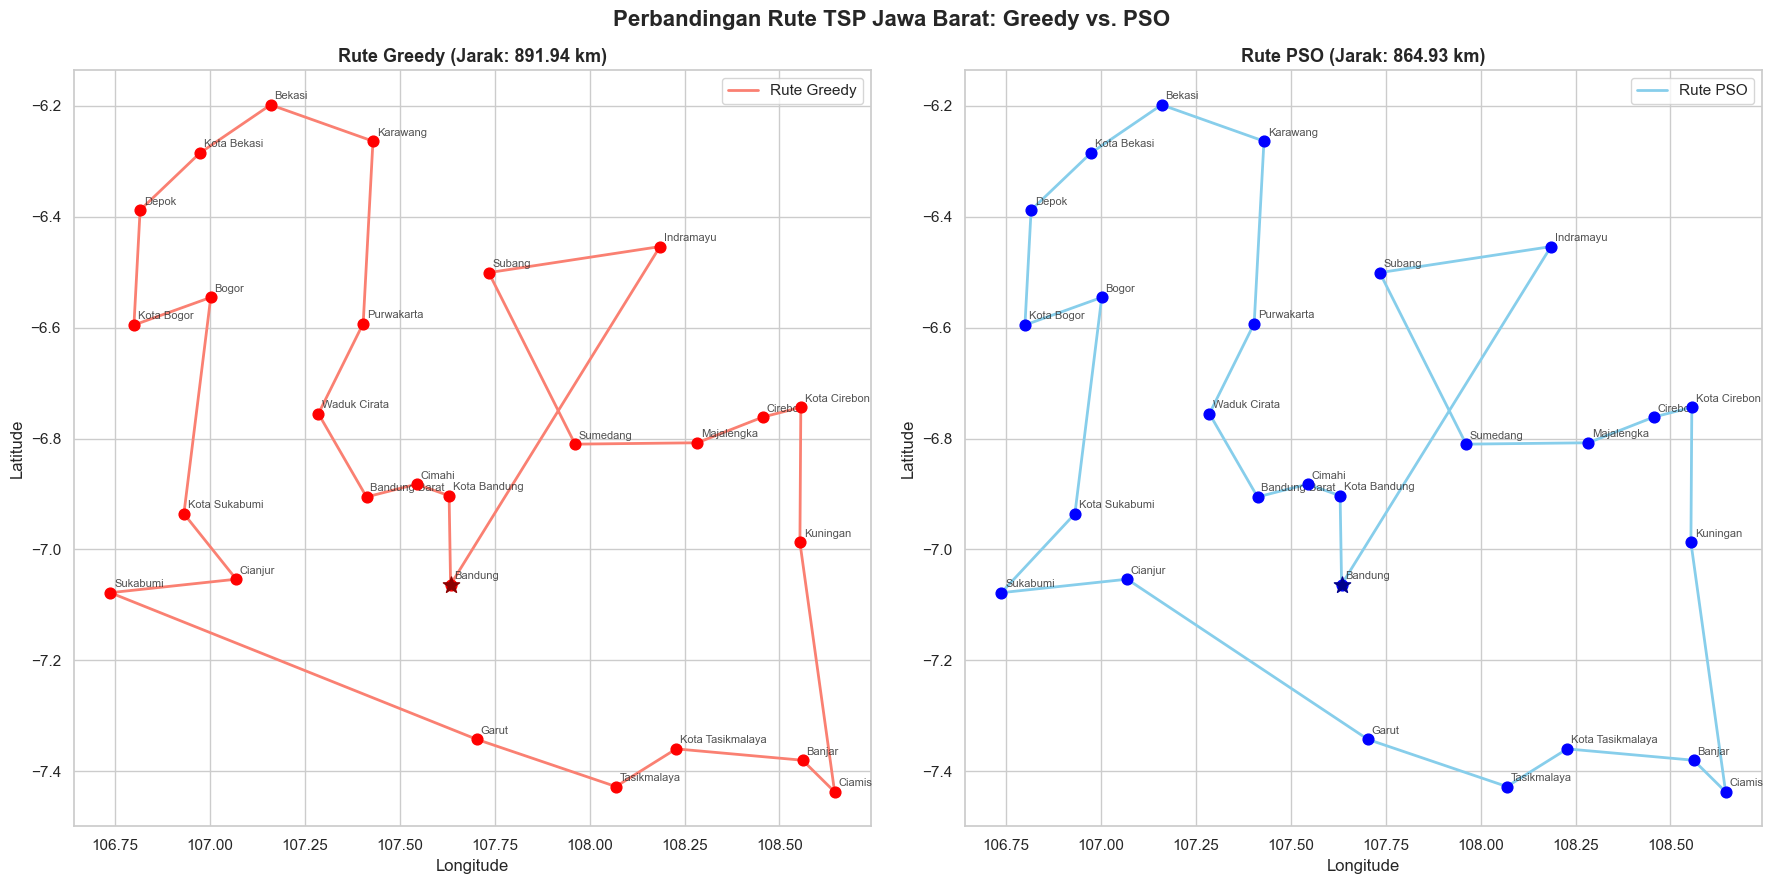
\includegraphics[width=\linewidth,height=0.74\textheight,keepaspectratio]{perbandingan_rute.png}
    {\scriptsize\color{Slate}
      Rute Greedy (kiri, merah) vs.\ rute PSO (kanan, biru) --- 27 kota Jawa Barat
    }

    \column{0.33\textwidth}
    \vspace{0.5cm}
    \begin{beamercolorbox}[wd=\linewidth,sep=8pt,rounded=true]{block body}
      \centering
      \pill{Rose}{Greedy}\\[5pt]
      {\Large\bfseries 891.94 km}
    \end{beamercolorbox}

    \vspace{0.20cm}
    \begin{beamercolorbox}[wd=\linewidth,sep=8pt,rounded=true]{block body}
      \centering
      \pill{Leaf}{PSO}\\[5pt]
      {\Large\bfseries 864.93 km}
    \end{beamercolorbox}

    \vspace{0.20cm}
    \begin{block}{Peningkatan}
      \centering
      {\LARGE\bfseries\color{Sky} $-$3.03\%}\\[2pt]
      {\small rute lebih pendek}
    \end{block}

    \vspace{0.18cm}
    {\footnotesize\color{Slate}
      Konvergen di iterasi ke-21\\(early stopping aktif)
    }
  \end{columns}
\end{frame}


% ─────────────────────────────────────────────
%  SLIDE 8 · Kurva Konvergensi PSO
% ─────────────────────────────────────────────
\begin{frame}{Kurva Konvergensi PSO}
  \framesubtitle{Insan Anshary Rasul · G6401231132}
  \begin{columns}[T,totalwidth=\textwidth]
    \column{0.65\textwidth}
    \centering
    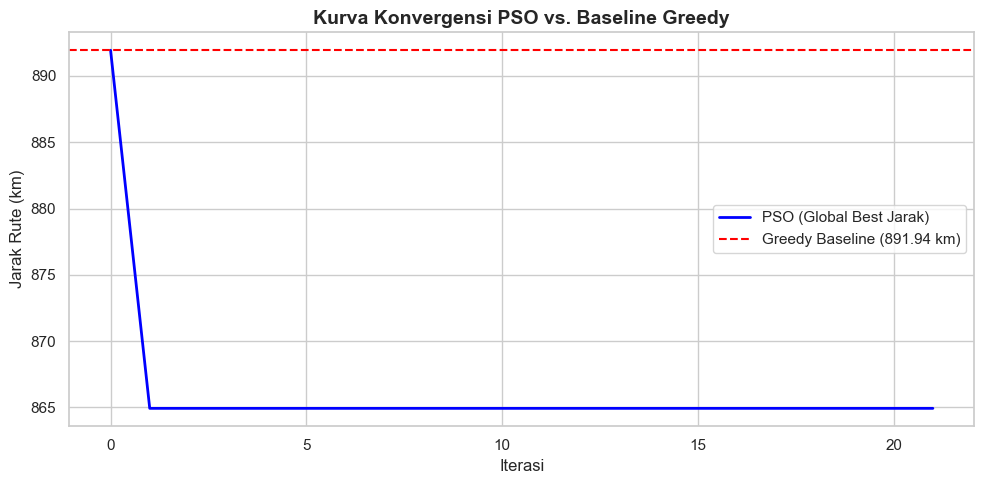
\includegraphics[width=\linewidth,height=0.74\textheight,keepaspectratio]{kurva_konvergensi_psi_vs_baseline_greedy.png}
    {\scriptsize\color{Slate}
      Jarak \textit{global best} PSO (biru) vs.\ baseline Greedy (merah putus-putus) per iterasi
    }

    \column{0.32\textwidth}
    \vspace{0.5cm}
    \begin{beamercolorbox}[wd=\linewidth,sep=8pt,rounded=true]{block body}
      \textbf{Yang Terjadi:}
      \begin{itemize}\small
        \item Jarak turun tajam di iterasi 0--2
        \item PSO \textbf{langsung} melampaui Greedy
        \item Plateau stabil sejak iterasi 2
        \item Konvergen total di iterasi \textbf{21}
      \end{itemize}
    \end{beamercolorbox}

    \vspace{0.25cm}
    \begin{block}{Kesimpulan Grafik}
      \small
      Kawanan 15 partikel menemukan
      solusi lebih baik dari Greedy
      \textbf{hanya dalam 2 iterasi pertama}.
    \end{block}
  \end{columns}
\end{frame}


% ─────────────────────────────────────────────
%  SLIDE 9 · Analisis Kinerja Akademik
% ─────────────────────────────────────────────
\begin{frame}{Analisis Kinerja Akademik}
  \framesubtitle{Insan Anshary Rasul · G6401231132}
  \begin{columns}[T,totalwidth=\textwidth]
    \column{0.65\textwidth}
    \centering
    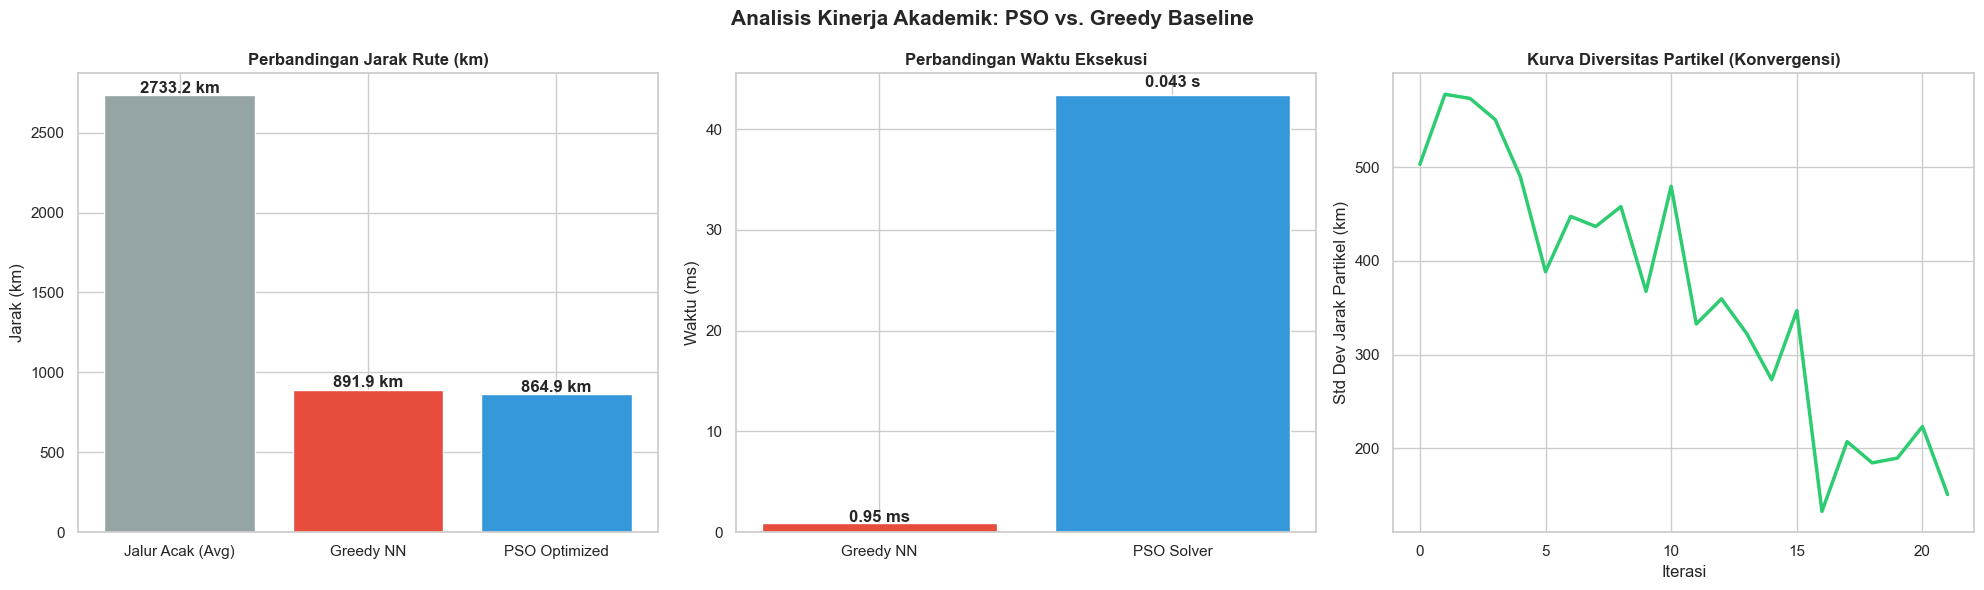
\includegraphics[width=\linewidth,height=0.74\textheight,keepaspectratio]{analisis_kinerja_akademik.png}
    {\scriptsize\color{Slate}
      Perbandingan jarak rute, waktu eksekusi, dan diversitas partikel (konvergensi)
    }

    \column{0.32\textwidth}
    \vspace{0.2cm}
    \begin{beamercolorbox}[wd=\linewidth,sep=8pt,rounded=true]{block body}
      \textbf{Panel Kiri --- Jarak:}\\[3pt]
      {\small PSO (864.9 km) jauh lebih baik dari rute acak (2733.2 km) dan lebih baik dari Greedy (891.9 km)}
    \end{beamercolorbox}

    \vspace{0.15cm}
    \begin{beamercolorbox}[wd=\linewidth,sep=8pt,rounded=true]{block body}
      \textbf{Panel Tengah --- Waktu:}\\[3pt]
      {\small Greedy 0.95 ms vs.\ PSO 43 ms\\\textit{trade-off} kecepatan vs.\ kualitas}
    \end{beamercolorbox}

    \vspace{0.15cm}
    \begin{beamercolorbox}[wd=\linewidth,sep=8pt,rounded=true]{block body}
      \textbf{Panel Kanan --- Diversitas:}\\[3pt]
      {\small Std.\ Dev.\ partikel turun $\Rightarrow$ kawanan menyatu ke solusi terbaik}
    \end{beamercolorbox}
  \end{columns}
\end{frame}


% ─────────────────────────────────────────────
%  SLIDE 10 · Matriks Jarak Geografis
% ─────────────────────────────────────────────
\begin{frame}{Analisis Spasial: Matriks Jarak Geografis}
  \framesubtitle{Daffa Naufal Mumtaz · G6401231168}
  \begin{columns}[T,totalwidth=\textwidth]
    \column{0.60\textwidth}
    \centering
    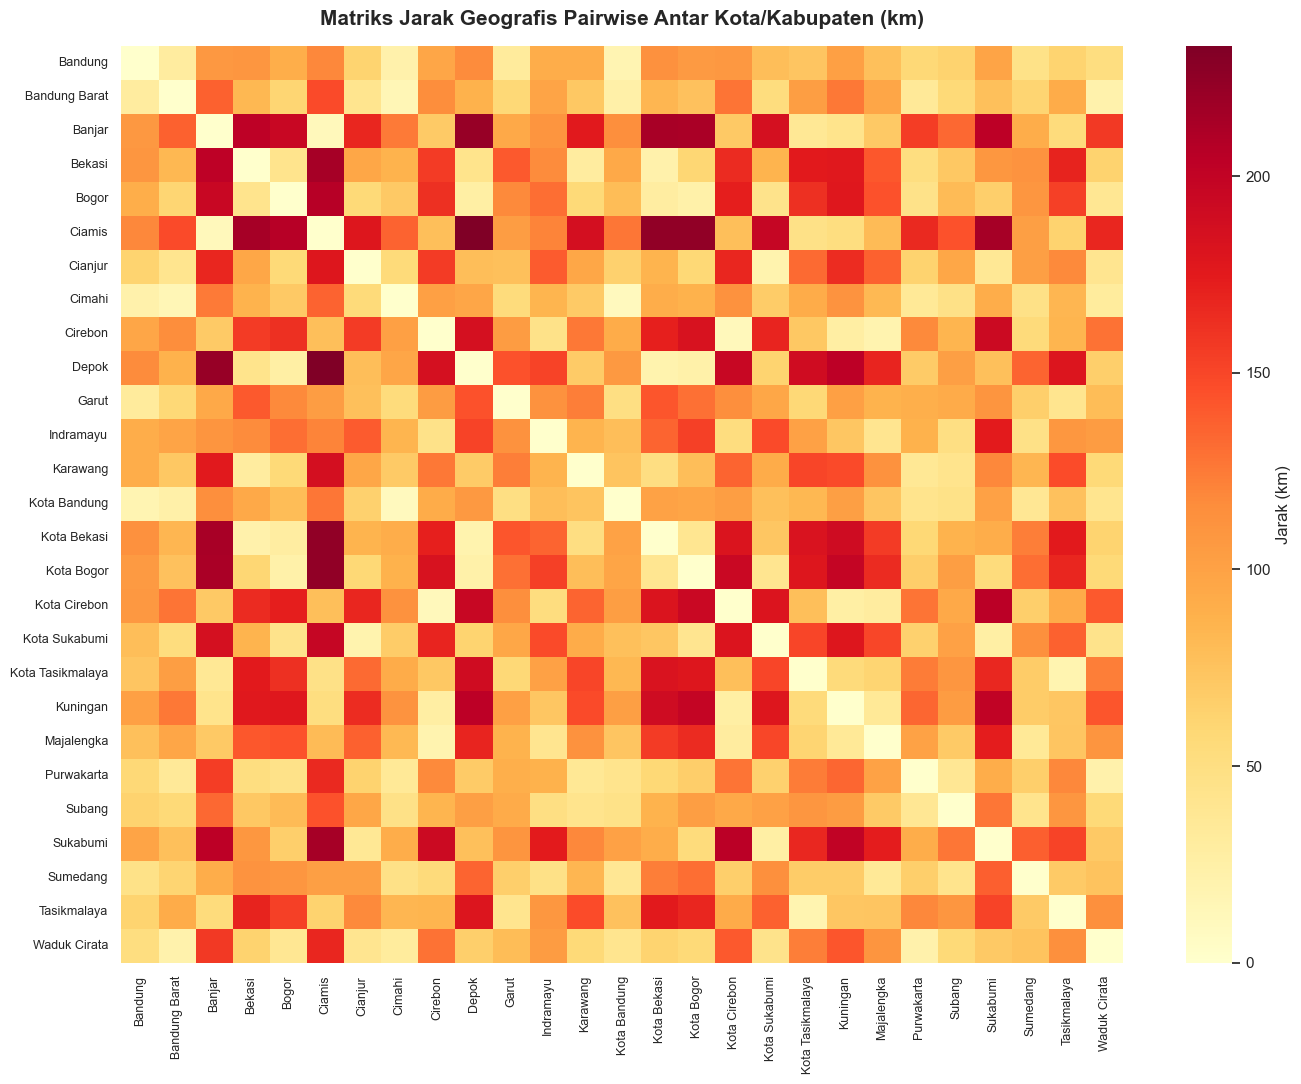
\includegraphics[width=\linewidth,height=0.74\textheight,keepaspectratio]{matriks_jarak_geografis.png}
    {\scriptsize\color{Slate}
      Heatmap jarak Haversine (km) pairwise antar 27 kota/kabupaten Jawa Barat
    }

    \column{0.37\textwidth}
    \vspace{0.2cm}
    \begin{beamercolorbox}[wd=\linewidth,sep=8pt,rounded=true]{block body}
      \textbf{Cara Membaca:}
      \begin{itemize}\small
        \item Warna merah $=$ jarak jauh
        \item Warna kuning $=$ jarak dekat
        \item Diagonal $= 0$ (kota ke dirinya)
        \item Simetris: $d_{ij} = d_{ji}$
      \end{itemize}
    \end{beamercolorbox}

    \vspace{0.2cm}
    \begin{block}{Insight Geografis}
      \small
      \begin{itemize}
        \item Cluster paling dekat:\\
              \textbf{Bandung Raya} (Bandung, Kota Bandung, Cimahi, Bandung Barat)
        \item Jarak terjauh: kota barat (Bogor/Depok) ke kota timur (Cirebon/Indramayu)
      \end{itemize}
    \end{block}

    \vspace{0.15cm}
    {\footnotesize\color{Slate}
      Matriks ini menjadi dasar perhitungan
      fungsi \textit{fitness} PSO.
    }
  \end{columns}
\end{frame}


% ─────────────────────────────────────────────
%  SLIDE 11 · Distribusi Panjang Langkah
% ─────────────────────────────────────────────
\begin{frame}{Distribusi Panjang Langkah (\textit{Edge Hop Length})}
  \framesubtitle{Daffa Naufal Mumtaz · G6401231168}
  \begin{columns}[T,totalwidth=\textwidth]
    \column{0.62\textwidth}
    \centering
    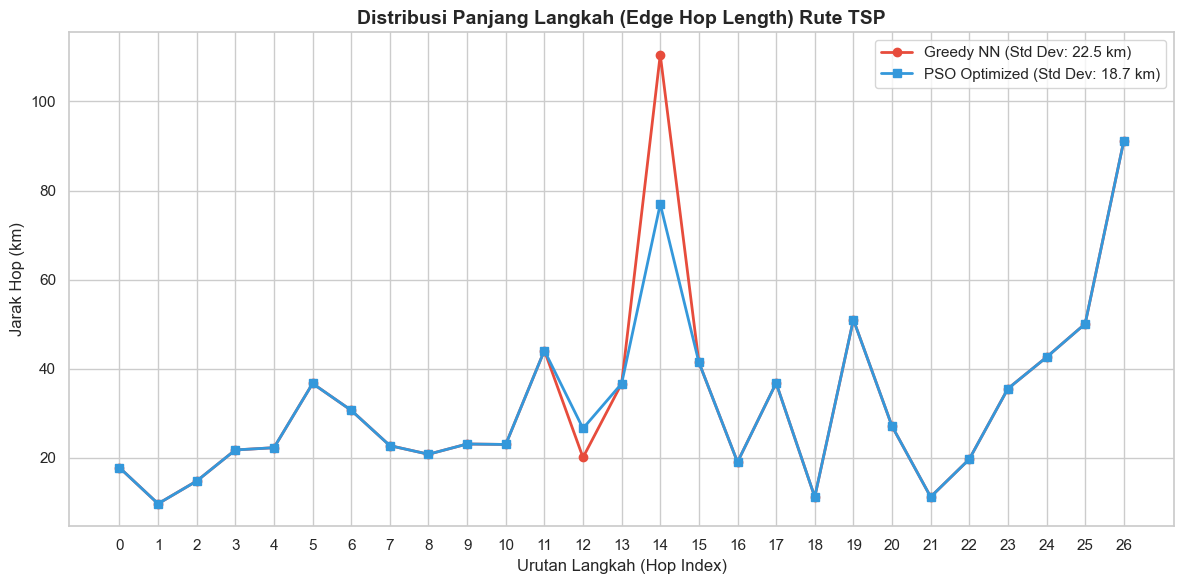
\includegraphics[width=\linewidth,height=0.72\textheight,keepaspectratio]{distribusi_panjang_langkah.png}
    {\scriptsize\color{Slate}
      Panjang tiap langkah (edge) pada rute Greedy (merah) vs.\ PSO (biru)
    }

    \column{0.35\textwidth}
    \vspace{0.3cm}
    \begin{block}{Interpretasi}
      \small
      \begin{itemize}
        \item Greedy Std.\ Dev.: \textbf{22.5 km}
        \item PSO Std.\ Dev.: \textbf{18.7 km}
        \item PSO lebih \textbf{konsisten} antar langkah
        \item Greedy membuat lompatan besar di hop ke-14 (${\approx}$110 km)
      \end{itemize}
    \end{block}

    \vspace{0.2cm}
    \begin{beamercolorbox}[wd=\linewidth,sep=8pt,rounded=true]{block body}
      \small\textbf{Bukti Keunggulan PSO:}\\[3pt]
      Distribusi hop lebih merata $=$ PSO memanfaatkan kedekatan geografis secara lebih efisien
    \end{beamercolorbox}
  \end{columns}
\end{frame}


% ─────────────────────────────────────────────
%  SLIDE 12 · Kesimpulan
% ─────────────────────────────────────────────
\begin{frame}{Kesimpulan}
  \framesubtitle{Daffa Naufal Mumtaz · G6401231168}
  \begin{columns}[T,totalwidth=\textwidth]
    \column{0.50\textwidth}
    \begin{block}{Hasil Utama}
      \begin{itemize}
        \item PSO menemukan rute \textbf{864.93 km} vs.\
              Greedy \textbf{891.94 km}
        \item Penghematan jarak: \textbf{3.03\%}
        \item Konvergen dalam \textbf{21 iterasi} berkat \textit{early stopping}
        \item Auto-tuning memilih:\\
              \textit{Exploitation-Heavy} ($w{=}0.4,\ c_2{=}2.0$)
        \item Diversitas partikel turun konsisten\\
              $\Rightarrow$ konvergensi terbukti secara akademik
      \end{itemize}
    \end{block}

    \column{0.47\textwidth}
    \sectiontitle{Ringkasan Perbandingan}
    \vspace{0.2cm}

    \begin{tabular}{@{}lcc@{}}
      \toprule
                          & \textbf{Greedy} & \textbf{PSO} \\
      \midrule
      Jarak               & 891.94 km    & \textbf{864.93 km} \\
      Waktu               & \textbf{0.95 ms} & 43.4 ms \\
      Kualitas rute       & Lokal           & \textbf{Global} \\
      Std.\ Dev.\ hop     & 22.5 km         & \textbf{18.7 km} \\
      \bottomrule
    \end{tabular}

    \vspace{0.3cm}
    \begin{beamercolorbox}[wd=\linewidth,sep=8pt,rounded=true]{block body}
      \small\textbf{Rekomendasi:}\\[3pt]
      Gunakan \textbf{PSO} untuk logistik/distribusi
      yang mengutamakan optimalitas rute.
      Gunakan \textbf{Greedy} untuk keputusan
      \textit{real-time} yang butuh kecepatan.
    \end{beamercolorbox}
  \end{columns}
\end{frame}


% ─────────────────────────────────────────────
%  SLIDE 13 · Penutup
% ─────────────────────────────────────────────
\begin{frame}[plain]
  \begin{tikzpicture}[remember picture,overlay]
    \fill[Ink] (current page.south west) rectangle (current page.north east);
    \fill[Sky]           ([xshift=-1.6cm,yshift=1.0cm]current page.south east) circle (1.35cm);
    \fill[white,opacity=0.08] ([xshift=1.8cm,yshift=-1.0cm]current page.north west) circle (2.0cm);
    \fill[Sky,opacity=0.25]   ([xshift=5.5cm,yshift=-1.8cm]current page.north west) circle (0.9cm);
  \end{tikzpicture}

  \vspace{1.8cm}
  \centering
  {\color{white}\Huge\bfseries Terima Kasih}

  \vspace{0.5cm}
  {\color{white!80}\large Sesi Tanya Jawab}

  \vspace{0.8cm}
  {\color{white!55}\footnotesize
    Naufal Akmal Rizqulloh\enspace$\cdot$\enspace
    Adhiya Radhin Fasya\enspace$\cdot$\enspace
    Faiz Naufal Huda\\[4pt]
    Insan Anshary Rasul\enspace$\cdot$\enspace
    Daffa Naufal Mumtaz
  }
\end{frame}

\end{document}
